\section{\txnimp}
\label{sec:syntax}

\subsection{\txnimp: Syntax and Semantics}
\label{sec:opsem}

\renewcommand{\ctxn}[3]{\C{TXN}_{#1}\langle #2 \rangle\{#3\}}
\begin{figure*}[!ht]
\raggedright
%
\textbf{Syntax}\\
%
\begin{smathpar}
\renewcommand{\arraystretch}{1.2}
\begin{array}{lclcl}
\multicolumn{5}{c} {
  {x,y} \in \mathtt{Variables}\qquad
  {f} \in \mathtt{Field\;Names} \qquad
% {\tau} \in \mathtt{Table\;Names}
  {i,j} \in \mathbb{N} \qquad
  {\odot} \in \{+,-,\le,\ge,=\}\qquad
}\\
\multicolumn{5}{c}{
  {k} \in \mathbb{Z}\cup\mathbb{B} \qquad
  {\rec} \in \{\bar{f}=\bar{k}\}\qquad
  {\stl,\stg,s} \in \Pow{\rec} \qquad
  \I \in \mathbb{B}\times\Pow{\rec}\times\Pow{\rec}\times\Pow{\rec}
  \rightarrow \Prop
}\\
v & \in & \mathtt{Values} & \coloneqq & k \ALT \rec \ALT s\\
e & \in & \mathtt{Expressions} & \coloneqq & c \ALT x \ALT x.f 
    \ALT \{\bar{f}=\bar{e}\} \ALT e_1 \odot e_2\\ 
c & \in & \mathtt{Commands} & \coloneqq & \cskip \ALT \lete{x}{e}{c}
    \ALT \ite{e}{c_1}{c_2}\ALT c_1;c_2 \ALT \inserte{e}  \\
&&&&\ALT \deletee{\lambda x.e}
    \ALT \lete{x}{\selecte{\lambda x.e}}{c}
    \ALT \updatee{\lambda x.e_1}{\lambda x.e_2}\\
&&&&\ALT \foreache{e_1}{\lambda x.\lambda y. e_2} 
    \ALT \foreachr{s_1}{s_2}{\lambda x.\lambda y. e}\\
&&&&\ALT \ctxn{i}{\I}{ c } \ALT \ctxn{i}{\I,\stl,\stg}{c} \ALT c1 || c2\\
% t & \in & \mathtt{Terms} & \coloneqq & e \ALT c\\
\ectx & \in & \mathtt{Eval\;Ctx} & ::= & \bullet \ALT  
  \bullet || c_2 \ALT c_1 || \bullet \ALT \bullet;\,c_2 
  \ALT \ctxn{i}{\I,\stl,\stg}{\bullet} \\
\end{array}
\end{smathpar}
%
\bigskip

\renewcommand{\arraystretch}{1.2}

%
\textbf{Local Reduction} \quad 
\fbox {\(\stg \vdash (c,\stl) \stepsto (c',\stl')\)}\\
%
\begin{minipage}{2.8in}
\rulelabel{E-Insert}
\begin{smathpar}
\begin{array}{c}
\RULE
{
  i \not\in \dom(\stl \cup \stg)\\
  r = \{\bar{f}=\bar{k};\,\idf=i;\,\delf=\C{false}\}
}
{
  \stg \vdash (\inserte{\{\bar{f}=\bar{k}\}},\stl) \stepsto
  (\cskip,\stl \cup \{r\})
}
\end{array}
\end{smathpar}
\end{minipage}
%
%
\begin{minipage}{2.8in}
\rulelabel{E-Delete}
\begin{smathpar}
\begin{array}{c}
\RULE
{
  s = \{r' \,|\, \exists(r\in\Delta).~ \eval([r/x]e)=\C{true} \\
        \hspace*{0.7in}\conj r'=\{\bar{f}=r.\bar{f}; \idf=r.\idf;
        \delf=\C{true}\}\}\\
% \dom(s) \cap \dom(\delta) = \emptyset
}
{
  \stg \vdash (\deletee{\lambda x.e},\stl) \stepsto (\cskip,\stl \cup s)
}
\end{array}
\end{smathpar}
\end{minipage}
%
\bigskip

%
\begin{minipage}{2.8in}
\rulelabel{E-Select}
\begin{smathpar}
\begin{array}{c}
\RULE
{
  s = \{r\in\Delta \,|\, \eval([r/x]e)=\C{true}\}\spc
  c' = [s/x]c
}
{
  \stg \vdash (\lete{x}{\selecte{\lambda x.e}}{c}, \stl) \stepsto 
              (c',\stl)
}
\end{array}
\end{smathpar}
\end{minipage}
%
%
\begin{minipage}{2.8in}
\rulelabel{E-Update}
\begin{smathpar}
\begin{array}{c}
\RULE
{
  s = \{r' \,|\, \exists(r\in\Delta).~ \eval([r/x]e_2)=\C{true} \conj r'=[r/x]e_1\}\\
}
{
  \stg \vdash (\updatee{\lambda x.e_1}{\lambda x.e_2},\stl) \stepsto 
              (\cskip,\stl \cup s)
}
\end{array}
\end{smathpar}
\end{minipage}
%

\begin{smathpar}
\begin{array}{ll}
  \rulelabel{E-Foreach1} & \stg \vdash (\foreache{e}{\lambda x.\lambda
  y.c},\stl) \stepsto (\foreachr{\emptyset}{\eval(e)}{\lambda x.\lambda y. c})\\
  \rulelabel{E-Foreach2} & \stg \vdash (\foreachr{s_1}{\{r\} \cup s_2}{\lambda x.\lambda
  y.c},\stl) \stepsto ([r/y][s_1/x]c;\,\foreachr{s_1 \cup \{r\}}{s_2}{\lambda x.\lambda y. c})\\
  \rulelabel{E-Foreach3} & \stg \vdash (\foreachr{s}{\emptyset}{\lambda x.\lambda
  y.c},\stl) \stepsto (\cskip,\stl)\\
\end{array}
\end{smathpar}
%
\bigskip

%
\textbf{Top-Level Reduction} \quad 
\fbox {\((c,\stg) \stepsto (c',\stg')\)}\\
%
\begin{minipage}{3in}
\rulelabel{E-Txn}
\begin{smathpar}
\begin{array}{c}
\RULE
{
  \I(\C{true},\stl,\stg,\stg')\spc
  \stg \vdash (c,\stl) \stepsto (c',\stl')
}
{
  (\ctxn{i}{\I,\stl,\stg}{c},\stg') \stepsto
  (\ctxn{i}{\I,\stl',\stg'}{c'},\stg')
}
\end{array}
\end{smathpar}
\end{minipage}
%
%
\begin{minipage}{2.8in}
\rulelabel{E-Commit}
\begin{smathpar}
\begin{array}{c}
\RULE
{
  \I(\C{false},\stl,\stg,\stg')
}
{
  (\ctxn{i}{\I,\stl,\stg}{\cskip},\stg') \stepsto (\cskip,\stl\gg\stg')
}
\end{array}
\end{smathpar}
\end{minipage}
%


\caption{\small \txnimp: Syntax and Small-step semantics}
\label{fig:txnimp}
\end{figure*}



Fig.~\ref{fig:txnimp} shows the syntax and small-step semantics of
\txnimp, a core language that we will use to formalize the intuitions
presented in the previous section. Natural numbers, (shared) variables
and arithmetic expressions constitute the syntactic class of
expressions ($e$).  Commands ($c$) include $\cskip$, assignment
statements, transaction (\C{txn}) lexical blocks, and their sequential
and parallel composition. We let $T_i$ for $i \in \mathbb{N}$ range
over transaction identifiers. When it is evident we are referring to a
transaction, we use the number $i$ instead of $T_i$ for identification
(\eg, in $\C{txn}\langle i \rangle$). For notational convenience, we
let $t$ range over both expressions and commands.

We define a small-step operational semantics for this language in
terms of an abstract machine that generates an execution trace
($\E$). The first component of the trace is a set ($\A$) of
\emph{effects}, where an effect ($\eta$) documents a read (\C{RD(X)}),
a write (\C{WR(X)}), or a transaction commit (\C{COMMIT}) operation
performed during the execution. Any value associated with the
operation (\eg, value read or value written) is also documented, and
can be accessed via $\rval$. Every effect has a unique identifier
accessible via $\id$, and a transction identifier accessible via
$\txn$.  The latter identifies the transaction that generated the
effect. In every step of the evaluation, the machine reduces a \txnimp
term by executing a read, write or commit operation, generating an
effect, and extending the trace. Since effects include transaction
identifiers, the semantics distinguishes between terms ($t$) of
different transactions. For example, $\txnbox{t}_i$ denotes a term $t$
inside a transaction $T_i$.  Evaluation contexts are also
appropriately marked. For example, $\ectx_i$ denotes the evaluation
context for a term inside $T_i$. The other component of an execution
trace is a visibility relation ($\visZ$) that establishes a visibility
property between effects among different transactions. The intent and
mechanics of $\visZ$ is described in the sequel.

Fundamental to our development is the notion of a trace invariant
($\I$). $\I$ is a function from traces ($\E$) to propositions
($\texttt{Prop}$) that define well-formedness constraints over traces.
The machine takes a step only if the resulting trace satisfies the
constraints imposed by $\I$. This behaviour is captured by the
auxiliary reduction rule \rulelabel{E-Aux} that factors out the trace
extension aspect of the evaluation by abstracting away the
operation-specific behaviour as a function that generates an
appropriate effect. We let $\mathcal{F}$ denote this function.
\rulelabel{E-Aux} uses $\mathcal{F}$ to generate a new effect and
extend the trace ($\E = (\A,\visZ)$) \emph{only if} the
well-formedness constraints imposed by $\I$ on $\E$ (i.e., $\I(\E')$)
are satisfied. Otherwise, it gets stuck. In an execution that runs to
completion, every small-step preserves the well-formedness of a trace,
thus ensuring the invariance of $\I$.  Note that the semantics makes
no assumptions about $\I$ other than its type. As such, it can be
instantiated with any trace-parametric proposition that expresses
constraints over the given trace. For instance, consider the
$\psi_{RC}$ specification from \S\ref{sec:motivation}, but with
bounded $T_1$ and $T_2$ instantiated with \C{Wd1} and \C{Wd2},
respectively. The instantiated specification is the following
proposition:

\begin{smathpar}
\begin{array}{l}
  \forall \eta_1,\eta_2,.\; \txn(\eta_1) = \C{Wd1}
  \conj \txn(\eta_2) = \C{Wd2} \\
  \hspace*{0.6in}\conj \C{Wd1} \neq \C{Wd2} \conj \eta_1 \hboar
  \eta_2 \Rightarrow \C{Wd1} \hboar \eta_2 \\
\end{array}
\end{smathpar}

\noindent It is easy to intepret the above proposition in the context of a trace
$\E$ that captures an execution of the program in
Fig.~\ref{fig:motiv-eg-1}. Such a trace-parametric proposition can be
used to instantiate the trace invariant $\I$ in Fig.~\ref{fig:txnimp}.
The resultant operational semantics describes an abstract machine that
gets stuck if an operation of \C{Wd2} is executed in a state that
incorporates some, but not all the effects (including the \C{COMMIT})
of \C{Wd1}. 
% While the machine takes a step only if the constraints are
% satisfied, it neither defines nor explicitly assumes an oracle to
% check satisfaction.

As described in \S\ref{sec:motivation}, the semantics of various
isolation levels can be captured as constraints over the
happens-before ($\hbZ$) relation. $\hbZ$ is however a derived relation
in our model, composed of more fundamental \emph{session order}
($\soZ$) and \emph{visibility} ($\visZ$) relations.  A session order
relation captures the sequential order of operations within a
transaction. In particular, it relates two effects, $\eta_1$ and
$\eta_2$, such that $\txn(\eta_1) = \txn(\eta_2)$ and $\id(\eta_1) <
\id(\eta_2)$.  The semantics assigns monotonically increasing
identifiers to effects, as defined by the $\id(\eta) > \maxId(\A)$
condition of \rulelabel{E-Aux}.  Evaluation contexts ($\ectx_i$) for
transaction-bound terms are defined so as to enforce a deterministic
sequential order of execution within a transaction, leading to a
deterministic total order among effect ids, which defines the session
order relation. Visibility ($\visZ$) on the other hand relates effects
across concurrent transactions.  Intuitively, $\visZ$ relates $\eta_1$
to $\eta_2$ if and only if $\eta_1$ was \emph{visible} to the
operation that generated $\eta_2$ during its execution, thus effecting
its return value ($\rval(\eta_2)$). For example, a read operation over
\C{X} may pick the value ($\rval$) of the write effect with highest id
among the visible effects (this is made possible by appropriately
defining $\interp{\cdot}$ in \rulelabel{E-Var}, as we show
later). Thus, the value of a read depends on what write effects it can
witness. An operation can only witness the effects of already
concluded operations, which varies between executions due to the
non-deterministic order of evaluating the parallel composition of
transactions. A more notable source of non-determinism, however, is
the \rulelabel{E-Aux} rule, which allows the machine to expose an
arbitrary subset ($S$) of existing effects ($\A$) to the incoming
operation. In other words, the machine is not obligated to reveal the
effects of all previous operations to an incoming operation. This
relaxation allows the abstract machine to model the semantics of
weakly consistent data stores. For instance, operations issued to an
eventually consistent (EC) replicated store could be dispatched to
different replicas whose states may not be in any well-defined
relationship. By allowing operations to witness arbitrary subsets of
the global state, the semantics models the weak visibility properties
of such stores.

However, a machine that lets operations witness arbitrary subset of
the global state offers no isolation whatsoever. For example, it may
allow a read operation to witness writes of an uncommitted
transaction, violating RC isolation. Fortunately, our ability to
express an isolation semantics as constraints over happens-before
order through $\visZ$ and $\soZ$ relations, and the property of the
abstract machine to be parametric over the trace invariant ($\I$),
lets us solve this problem.  In particular, we continue to define
isolation semantics as constraints over $\visZ$ and $\soZ$, but
confine their domain of interpretation to the given trace so that they
now become trace well-formedness constraints. Well-formedness
constraints can be combined into a trace invariant ($\I$). Since the
abstract machine is guaranteed to preserve $\I$ at every step of the
execution, operations are guaranteed to experience the level of
isolation specified by $\I$.  Thus, in executions that run to
completion, the abstract machine models a store that provides the
required levels of isolation. Notably, the machine achieves this
without defining an operation semantics for isolation levels, solely
by relying on their declarative characterization as trace
well-formedness constraints.  \S\ref{sec:ansi-isolation} shows the
specification of various ANSI SQL isolation levels stated as trace
well-formedness constraints.

As described previously, \rulelabel{E-Aux} abstracts away the
operation-specific behaviour of a machine step as a function ($\F$)
that accepts a set ($S$) of effects chosen by the machine to make
visible to the operation, interprets the operation w.r.t $S$, and
returns an appropriate effect that encodes its return value. Rules
\rulelabel{E-Var}, \rulelabel{E-Asgn} and \rulelabel{E-Commit} define
such functions for read, write and commit operations, respectively.
The effect returned by the function in each case includes its
transaction id ($T_i$) along with an arbitrarily chosen effect id
($j$) that is later verified to be unique in \rulelabel{E-Aux}. The
$\rval$ for a write is the value being written, and for commit it is
$\bot$. In case of a read, the value read depends on the how the read
operation chooses to interpret the given set ($S$) of visible effects.
The interpretation may depend on the application semantics. For
example, a monotonically increasing counter application may choose to
let a write with the largest value determine the value of a
read. A more straightforward interpretation has already been described
before. To accommodate multiple interpretations, the semantics
is made parametric over an interpretation function ($\interp{\cdot}$)
that accepts a set of effects and a variable name, and returns the
value associated with the variable. A straightforward interpretation
function that chooses the last write (i.e., write with largest id) is
shown below:

\begin{smathpar}
\begin{array}{lcl}
  \isMax(S,\eta) & \Leftrightarrow &  \forall (\eta'\in S).  
  \kind(\eta') = \kind(\eta) \\
  & & \hspace*{0.4in}\Rightarrow \eta' = \eta \disj \id(\eta') < \id(\eta)\\

\interp{S}(X) & = & \C{if}\;(\exists (\eta \in S). \kind(\eta) = \C{WR}(X) 
  \wedge \isMax(S,\eta)) \\
  & & \C{then}\;\rval(\eta)\;\C{else}\;0\\
\end{array}
\end{smathpar}

\noindent Rules \rulelabel{E-Top-Ctx} and \rulelabel{E-Txn-Ctx} define
congruence properties for top-level terms and transaction-bound terms,
respectively. The rules and evaluation contexts ($\ectx$ and
$\ectx_i$) are defined such that only certain kinds of terms are
allowed at the top-level and inside a transaction. In particular, a
\txnimp program at the top-level can either be a transaction, or a
parallel composition of transactions. A command inside a \C{txn} block
can either be an assignment, or a sequential composition of
assignments. 

\subsection{Specifications}
\label{sec:ansi-isolation}


% ISOLATION SPECS
% ---------------
\begin{figure*}[t!]
\begin{smathpar}
\begin{array}{lcl}
\underE{\C{RMWVis}(T_j)} & \defeq & \forall\eta_1,\eta_2.\,
       \underE{\{\eta_1,\eta_2\} \subseteq T_j} \conj
       \underE{\eta_1 \soar \eta_2} \Rightarrow \underE{\eta_1 \visar
       \eta_2}\\
\underE{\C{MonotonicVis}(T_j)} & \defeq & 
       \underE{\C{RMWVis}(T_j)} \conj 
       \forall\eta,\eta_1,\eta_2.\, \underE{\{\eta_1,\eta_2\} \in T_j} 
          \conj \\
  &   & \hspace*{1.2in}\underE{\eta \visar \eta_1} \conj
        \underE{\eta_1 \soar \eta_2} \Rightarrow \underE{\eta \visar
        \eta_2} \\
%  \C{CausalVis}(T_i) & \defeq & 
%         \C{MonotonicVis}(T_i) \conj \C{RMWVis}(T_i)\\
\underE{\C{AtomicVis}(T_j)} & \defeq & 
       \forall\eta_1,\eta_2.\, \neg(\underE{\eta_1 \in T_j}) \conj
       \underE{\eta_2 \in T_j} \conj
       \underE{\eta_1 \visar \eta_2} \Rightarrow \underE{\txn(\eta_1)
       \visar \eta_2}\\
\underE{\C{CommitVis}(T_j)} & \defeq & 
       \forall\eta_1,\eta_2.~ \neg(\underE{\eta_1 \in T_j}) \conj 
          \underE{\eta_2 \in T_j} \conj
       \underE{\eta_1 \visar \eta_2} \Rightarrow\\
  &   & \hspace*{1.2in}\exists\eta.\, \underE{\eta \in \txn(\eta_1)} 
        \conj \kind(\eta) = \C{COMMIT} 
        \conj \underE{\eta \visar \eta_2}\\
% \underE{\C{TransVis}(T_j)} & \defeq &  \forall
%        \eta_1,\eta_2,\eta_3.\, \underE{\eta_3 \in T_j} \conj
%        \underE{\eta_1 \visar \eta_2} \conj
%        \underE{\eta_2 \visar \eta_3} \Rightarrow \underE{\eta_1 \visar
%        \eta_3} \\
\underE{\C{RC}(T_j)} & \defeq & \underE{\C{AtomicVis}(T_j)} 
        \conj \underE{\C{CommitVis}(T_j)}\\
\underE{\C{MAV}(T_j)} & \defeq & \underE{\C{RC}(T_j)} \conj
      \underE{\C{MonotonicVis}(T_j)} \\
\underE{\C{SnapshotVis}(T_i,T_j)} & \defeq &  \underE{T_i
       \visar T_j} \disj \underE{T_i \invisar T_j}\\
\underE{\C{RR}(T_j)} & \defeq & \underE{\C{MAV}(T_j)}
       \conj \forall T_i.\,T_i \neq T_j \Rightarrow 
        \underE{\C{SnapshotVis}(T_i,T_j)} \\
% &   & \hspace*{2in}\conj  \C{SnapshotVis}(T_i,T_j)\\
\underE{\C{SnapshotSER}(T_i,T_j,X)} & \defeq &  \underE{T_i
       \visar T_j} \disj (\underE{T_i \invisar T_j} \conj \\
  &   &\hspace*{1.2in}\exists \eta.~\underE{\eta\in T_i} \conj \kind(\eta) =
       \C{WR(X)} \Rightarrow \underE{T_j \visar \eta})\\
\underE{\C{SI}(T_j)} & \defeq &  \underE{\C{RR}(T_j)}
       \conj \forall T_i.\,(T_i \neq T_j \conj \exists X.\, \underE{T_i \wrstoar X} \conj 
        \underE{T_j \wrstoar X})\\
%      (\exists X.\, T_i \wrstoar X \conj T_j \wrstoar X)
%      \Rightarrow  \C{TotalVis}(T_i,T_j)\\
  &   & \hspace*{2in} \Rightarrow \underE{\C{SnapshotSER}(T_i,T_j,X)}\\
\underE{\C{SER}(T_j)} & \defeq & \underE{\C{RR}(T_j)}
        \conj \forall T_i.\,(T_i \neq T_j \conj \exists X.\, 
        \underE{T_i \wrstoar X} \conj \underE{T_j \usesar X})\\
  &   & \hspace*{2in} \Rightarrow \underE{\C{SnapshotSER}(T_i,T_j,X)}\\
\end{array}
\end{smathpar}

\caption{Standard isolation guarantees expressed as trace
well-formedness constraints}
\label{fig:ansi-isolation}
\end{figure*}




We now describe specifications of standard isolation guarantees
expressed as constraints over trace well-formedness. For brevity and
convenience, we introduce some notations that are used in the following
sections.  An execution trace is destructed as ($\A$,$\visZ$) whenever
individual components of the pair are needed. Otherwise, it is written
as $\E$.  Sometimes, the dot notation (\eg~$\E.\A$) is also
used. Since $\A$ and $\visZ$ are both sets, we lift the operations on
sets to pairs of sets when updating $\E$. For example, $\E' = \E \cup
(\{\eta_2\},\{(\eta_1,\eta_2)\})$ expands to $\E' = (\E.\A \cup
\{\eta_2\},\,\E.\visZ \cup \{(\eta_1,\eta_2)\})$.  When $\psi$ is a
formula, $\underE{\psi}$ denotes the interpretation of $\psi$ in the
context of the trace $\E$. Such interpretations are defined on a
case-by-case basis in Figs.~\ref{fig:rel-defs}
and~\ref{fig:ansi-isolation}.

\subsubsection{Trace Relations}

Fig.~\ref{fig:rel-defs} shows various relations defined over elements
in a trace. In the context of a trace $(\A,\visZ)$, an effect $\eta$
is said to belong to a transaction $T_i$ if $\eta$ belongs to the
effect set $A$ and its transaction identifier is $T_i$. The
containment relation is trivially lifted to the set of effects to
define $\underE{S \subseteq T_i}$.  Visibility, session order, and
happens-before relations are denoted by $\eta_1 \visar \eta_2$,
$\eta_1 \soar \eta_2$, and $\eta_1 \hboar \eta_2$, respectively. A
transaction $T_i$ is said to be visible to an effect $\eta$ if every
effect $\eta_1$ of $T_i$ recorded by the trace is visible to $\eta$.
$T_i$ may be visible to $\eta$ but may not be visible to every other
effect in the $\txn(\eta)$. For a transaction $T_i$ to be considered
to be visible to a transaction $T_j$ in the context of a trace $\E$
(written $\underE{T_i \visar T_j}$), every effect ($\eta_1$) of $T_i$
present in $\E$ must be visible to every effect ($\eta_2$) of $T_j$ in
$\E$.  Conversely, if none of the effects of $T_i$ present in $\E$ are
visible to any effect of $T_j$, then $T_i$ is considered invisible to
$T_j$ under $\E$ (written $\underE{T_i \invisar T_j}$). Transaction
$T_i$ is said to have written to a variable $X$ under $\E$ (i.e.,
$\underE{T_i \wrstoar X}$) if there exists a $\C{WR}(X)$ effect from
$T_i$ in $\E$.  \emph{Reads-from} ($\underE{T_i \rdsfmar X}$) is
defined similarly. $T_i$ \emph{uses} $X$ ($T_i \usesar X$) if it reads
or writes $X$.

Fig.~\ref{fig:ansi-isolation} shows various isolation guarantees
defined as propositions indexed by transaction identifiers.
Transaction $T_j$ is said to have experienced \emph{read-my-writes}
visibility under $\E$ if every effect ($\eta_1$) of $T_j$ is visible
to every subsequent effect ($\eta_2$) of the same transaction in $\E$.
This lets $T_j$ to never lose its own updates. Monotonic visibility
adds one more constraint to \emph{read-my-writes}; besides requiring $\eta_1$
to be visible to $\eta_2$, it also requires every effect ($\eta$)
visible to $\eta_1$ in $\E$ to be visible to $\eta_2$ as well. Thus,
later operations in a transaction witness at least the same set of
effects witnessed by the earlier operations, if not more (hence,
``monotonic'' visibility). Atomic visibility allows an effect
$\eta_2$ of $T_j$ to witness an effect $\eta_1$ of $T_i$ only if all
effects of $T_i$ in $\E$ are also visible to $\eta_2$. Atomic
visibility thus prevents a transaction from being partially visible.
However, atomic visibility does not prevent an uncommitted transaction
from being visible. This is addressed by \C{CommitVis}, which requires
the commit effect of $T_i$ to be visible whenever any effect of $T_i$
is visible.

\subsubsection{Isolation Levels}

Fig.~\ref{fig:ansi-isolation} shows specifications of various
well-known isolation guarantees.  The ANSI SQL 92 standard requires
\iso{Read Committed} isolation to avoid the dirty reads phenomenon,
which is achieved by enforcing $\mathtt{AtomicVis}$ and
$\mathtt{CommitVis}$ guarantees. The {\sc rc} specification
(\C{RC})\footnote{In the following, we use small caps to abbreviate
isolation levels (\emph{e.g.,} {\sc rc} for \emph{Read Committed}),
and typewriter font for abbreviations of the specification of an
isolation level (\emph{e.g.,} \C{RC} denotes the specification for
{\sc rc} as given in Fig.~\ref{fig:ansi-isolation}).} is therefore a
combination of these two guarantees. The specification also agrees
with the description and implementation~\cite{bailishat,pldi15} of
{\sc rc} for highly available replicated stores. On relational
databases, however, {\sc rc} has also come to be associated with the
$\mathtt{MonotonicVis}$ guarantee.  Nonetheless, $\mathtt{AtomicVis}$
and $\mathtt{CommitVis}$ are sufficient to reason about {\sc rc}
isolation on relational stores too. The combination of these
guarantees with the {\sc sc} property of relational stores (formalized
in \S\ref{sec:store-consistency}) automatically leads to the
monotonicity guarantee, which explains why {\sc rc} comes with
$\mathtt{MonotonicVis}$ on such stores regardless of the
implementation. On weakly consistent stores however,
$\mathtt{AtomicVis}$ and $\mathtt{CommitVis}$ do not imply
$\mathtt{MonotonicVis}$. A stronger isolation level called
\iso{Monotonic Atomic View} ({\sc mav} of
Fig.~\ref{fig:ansi-isolation})~\cite{bailishat} was proposed to
explicitly extend {\sc rc} with monotonicity on such stores. 


Snapshot visibility (\C{SnapshotVis}) captures the scenario where a
transaction executes against a static snapshot of the database.  A
transaction $T_i$ is said to be snapshot-visible to a transaction
$T_j$ if either it is visible to $T_j$ (i.e., $T_i$ is included in the
snapshot), or it is invisible (i.e., it is not included); it is
forbidden for only a suffix (more generally, a subset) of $T_j$ to
witness $T_i$. The specification of ANSI SQL \iso{Repeatable Read}
isolation (\C{RR}) extends \C{MAV} with the snapshot visibility
guarantee.  Observe that snapshot visibility permits $T_i$ and $T_j$
to execute and commit while being oblivious of each other. This
scenario is captured in Fig.~\ref{fig:ansi-iso-eg-rr}, where
transactions $T_1$ and $T_2$, which perform conflicting writes,
execute against a snapshot of the database and commit concurrently.
While the actual values read and written by $T_1$ and $T_2$ are
unimportant (hence, elided), it is important to note the
\emph{absence} of visiblity arrows from $T_2$ to $T_1$, although $T_2$
commits before $T_1$'s read-from-$Y$.

\iso{Snapshot Isolation} ({\sc si}) proscribes this possibility. If
$T_i$ and $T_j$ both write to the same shared variable, then {\sc si}
insists that either $T_i$ be visible to $T_j$, or $T_j$ be visible to
the conflicting write of $T_i$ (this is captured by the auxiliary
definition \C{SnapshotSER}). Fig.~\ref{fig:ansi-iso-eg-si} shows an
execution where {\sc si} transaction $T_1$ witnesses a snapshot of the
database that doesn't include $T_2$. Due to \C{SI($T_1$)}, the
conflicting write to $X$ in $T_2$ is now required to witness $T_1$, as
captured by the direction of the $\visZ$ arrow (subsequent operations
also witness $T_1$ because $T_2$ is executing under {\sc mav}).
Lastly, \iso{Serializable} isolation extends $\mathtt{SnapshotSER}$ to
also cover non-conflicting transactions that write to variables read
in the current transaction.  Fig.~\ref{fig:ansi-iso-eg-ser} shows an
execution of an {\sc ser} transaction $T_3$ and a {\sc mav}
transaction $T_4$, which write to $X$ and $Y$, respectively. The
snapshot witnessed by the {\sc ser} transaction $T_3$ does not include
$T_4$, but the write to $Y$ in $T_4$, although non-conflicting,
witnesses $T_1$ because $Y$ is read by $T_1$. Visibility includes
other operations of $T_4$ because of {\sc mav}. Note that {\sc ser}
does not guarantee a total order on transactions w.r.t. $\visZ$
because, in practice, databases do not guarantee global serializable
execution unless \emph{all} transactions choose {\sc ser}.

\begin{figure}
\centering
\subcaptionbox {
  {\sc rr}($T_1$), {\sc rr}($T_2$).
  \label{fig:ansi-iso-eg-rr}
} [
  0.33\columnwidth
] {
  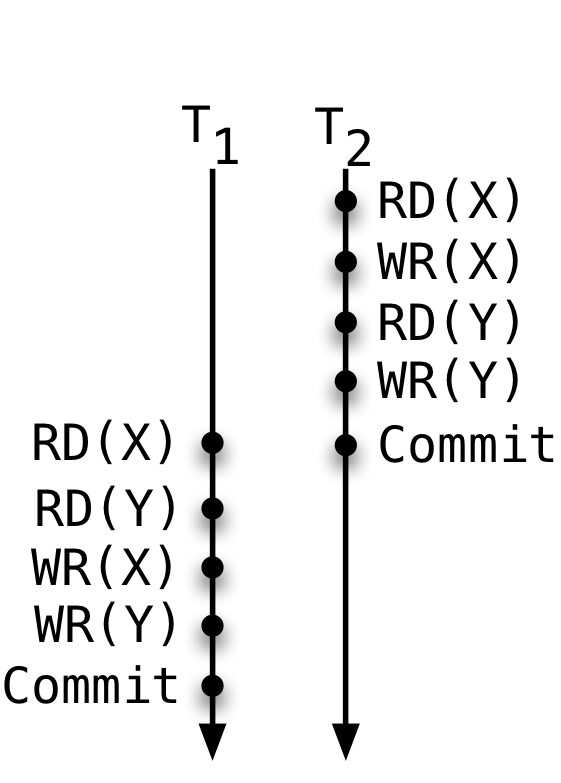
\includegraphics[scale=0.36]{Figures/rr-eg}
}
\subcaptionbox {
  {\sc si}($T_1$), {\sc mav}($T_2$)
  \label{fig:ansi-iso-eg-si}
} [
  0.33\columnwidth
] {
  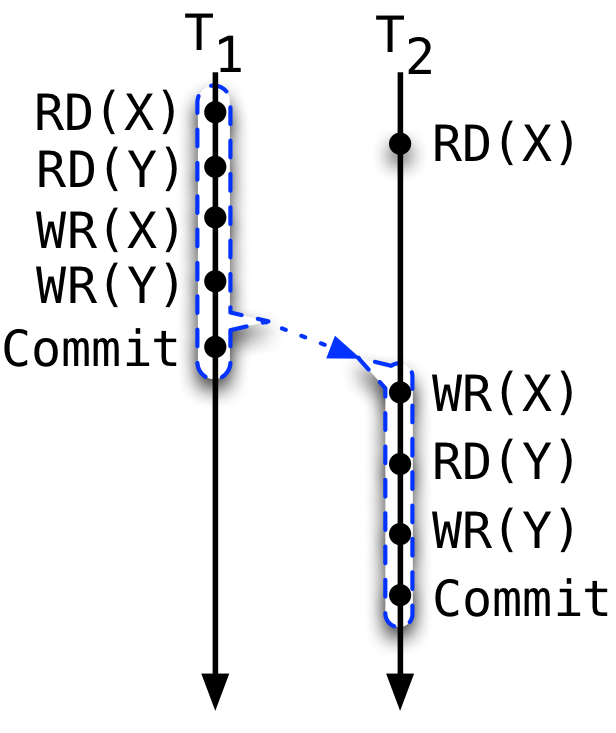
\includegraphics[scale=0.36]{Figures/si-eg-2}
}
\subcaptionbox {
  {\sc ser}($T_3$), {\sc mav}($T_4$)
  \label{fig:ansi-iso-eg-ser}
}{
  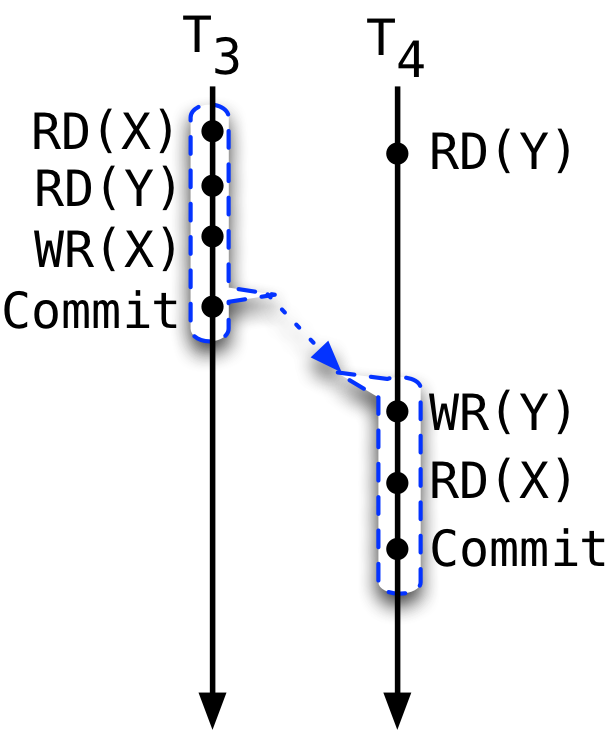
\includegraphics[scale=0.32]{Figures/ser-eg}
}

\caption{\small Sample executions of concurrent transactions at different
isolation levels. Solid (black) arrows indicate the timeline. Points
on the timeline mark the time when an operation is executed. Dotted
(blue) arrows denote $\visZ$. }
\label{fig:ansi-iso-eg}
\vspace*{-12pt}
\end{figure}

% Note that both $\mathtt{SnapshotVis}$ and $\mathtt{OneWaySER}$
% are asymmetric definitions that guarantee complete visiblity or
% invisibility of $T_i$ to $T_j$, but not the converse. While
% $\mathtt{SnapshotVis}$ provides no guarantees to $T_i$,
% $\mathtt{OneWaySER}$ guarantees that at least the commit effect of
% $T_i$ witnesses $T_j$. 

% \iso{Snapshot Isolation} spec ({\sc si}) extends {\sc rr} with a
% one-way serializability guarantee w.r.t. the transactions that perform
% conflicting writes (i.e., writes to the same shared variable).
% \footnote{Fig.~\ref{fig:ansi-isolation} presents slightly
% weaker versions of {\sc si} and {\sc ser} specs in the interest of
% clarity.}. Fig.~\ref{fig:ansi-iso-eg} shows sample executions of
% transactions $T_1$ and $T_2$. Both transactions read and write to
% shared variables $X$ and $Y$. In the first execution, $T_2$ commits
% while $T_1$ is still in progress, but {\sc rr} isolation prevents
% $T_1$ from witnessing the writes of $T_2$. In the second execution,

%% SJ: Not sure this paragraph is necessary here.
%% In contrast to recent proposals (\emph{e.g.},
%% ~\cite{gotsmanconcur15}), our specifications for {\sc si} and {\sc
%%   ser} do not necessarily impose a total order among transactions
%% (conflicting or otherwise). In reality, a total order under {\sc ser}
%% (resp. {\sc si}) is guaranteed only if the store executes all
%% transactions under {\sc ser} (resp. {\sc si}) isolation. Our
%% specifications admit this possibility, and derive a total order under
%% the assumption of homogenity. However, databases almost always allow
%% isolation levels to be configured on a per-transaction basis, allowing
%% transactions at various isolation levels to coexist.  Specifications
%% that assume homogenity are incorrect under this setting.

% Having specified isolation levels as trace well-formedness
% constraints, we can now construct trace invariants ($\I$) for
% \txnimp programs by composing isolation specifications for various
% transactions. For instance, the following trace invariant enforces
% {\sc si} for both transactions of the program in
% Fig.~\ref{fig:motiv-eg-1}, allowing it to satisfy its postcondition:
% \begin{smathpar}
% \I \;=\; \lambda\E.~ \underE{\C{SI(Wd1)}} \conj \underE{\C{SI(Wd2)}}
% \end{smathpar}
% In contrast, the following trace invariant enforces {\sc rc} for one and {\sc si}
% for another, leading to a possible violation of the postcondition:
% \begin{smathpar}
% \I \;=\; \lambda\E.~ \underE{\C{RC(Wd1)}} \conj \underE{\C{SI(Wd2)}}
% \end{smathpar}


\section{Data Stores and Consistency}
\label{sec:store-consistency}

The operational semantics of Fig.~\ref{fig:txnimp} allows operations
to witness arbitrary subsets of the global state, effectively mimicking the
behaviour of an eventually consistent ({\sc ec}) data
store\footnote{Eventual consistency guarantees that in the absence of further
  updates, all reads witness the same global state
  \emph{eventually}. In any finite trace, however, there are no
  guarantees on what a read may witness.}. There are, however, data stores,
such as relational databases, that provide stronger consistency
guarantees than {\sc ec}. Like the isolation levels of transactions,
the consistency level of the underlying store also affects the
semantics of a program in non-trivial ways. In this section, we
demonstrate how the semantics of stronger stores with on-demand weak
isolation can be captured in our operational model. 

% A non-trivial $\I$ composed of isolation specifications from
% Fig.~\ref{fig:ansi-isolation} induces the machine to provide
% non-trivial isolation guarantees for transactions. However, weak
% isolation levels often only constrain the visibility sets of
% operations by dictating what \emph{not} to see; not what to see.  For
% instance, \iso{Repeatable Read} isolation prohibits operations of a
% transaction from witnessing different states. It, however, does not
% prohibit all operations of a transaction from witnessing an aribitrary
% subset of the global state. Consequently, the machine can remain an
% {\sc ec} store even while providing non-trivial isolation. How then to
% model the semantics of an {\sc sc} store, such as a relational
% database, with variable (weak) isolation?

First, we observe that the semantics of a weakly-consistent data store
can be captured by store-specific consistency constraints, along with
transaction-specific isolation constraints, via the trace invariant
$\I$. In particular, we can split $\I$ into two components: (1).
$\I_s$, the store-specific invariant, and (2). $\I_c$, the
program-specific (or, client-specific) invariant, to capture
consistency and isolation constraints, resp.  $\I$ is now a
conjunction: $\I \,=\, \lambda\E.~\I_s(\E) \wedge \I_c(\E)$ (often
simplified to $\I \,=\, \I_s\wedge\I_c$).  While the program-specific
trace invariant ($\I_c$) remains an invariant regardless of the
specific consistency and visibility features exposed by the underlying
data store, the store specific invariant ($\I_s$) changes from store
to store depending on the consisteny level.  For an eventually
consistent store, $\I_s$ is simply \emph{true}. Stronger stores, such
as those that support strong consistenty, have non-trivial definitions
for $\I_s$.

A strongly-consistent {\sc sc} store guarantees a total order on all
operations w.r.t $\visZ$ consistent with their chronological order. A
straightforward $\I_s$ for this store is the \C{SC} property
formalized below:
\begin{smathpar}
\begin{array}{l}
  \C{sc}(\E) \;=\; \forall\eta_1,\eta_2.~\{\eta_1,\eta_2\}
  \subseteq \E.\A \conj \id(\eta_1) < \id(\eta_2) \\
  \hspace*{2in}\Rightarrow \underE{\eta_1 \visar \eta_2}
\end{array}
\end{smathpar}
Unfortunately, $\I_s=\C{SC}$ conflicts with all isolation
specifications of Fig.~\ref{fig:ansi-isolation}. For instance,
consider a case where $\I_c(\E) \;=\; \forall
T_i.~\underE{\C{RC}(T_i)}$, a constraint that dictates all
transactions execute under \iso{Read Committed} isolation. Imagine a
sample execution where $\eta_1$'s transaction is not yet committed
when $\eta_2$ is generated. Letting $\eta_1$ be visible to $\eta_2$
violates $\I_c$, whereas not letting it be visible violates $\I_{s}$.
The only way to satisfy both invariants is to rule out all 
executions that interleave the operations of one transaction with the
other, thereby enforcing serializability.  In general, when $\I_s$ conflicts (but is not
inconsistent) with $\I_c$, the only way to enforce both invariant sets
is to restrict concurrency. Clearly, this is unacceptable since it
defeats the very purpose of supporting weak isolation. 
% How then do we enforce weak isolation on a strongly consistent
% machine?

In practice, relational databases resolve such conflicts by
prioritizing weak isolation (thus, concurrency and performance) over
strong consistency, so the execution traces do not necessarily satisfy
{\sc sc}. In particular, visibility constraints imposed by {\sc sc}
are violated iff they are found to be in conflict with the constraints
imposed by a transaction's isolation level. In the context of
the aforementioned example, $\eta_1$ is not made visible to $\eta_2$
because doing so would violate $\I_c$. However, if $\I_c$ is true,
then the store makes $\eta_1$ visible to $\eta_2$ to honor its
consistency commitment\footnote{The term \emph{recency
    commitment}~\cite{bailishat} is often used in practice
  to capture the best-effort nature of {\sc sc}.}. We generalize this
approach to any $\I_s$ and $\I_c$ by defining a \emph{maximum
  visiblity principle} to determine an acceptable weakening of $\I_s$
in case of a conflict with $\I_c$.  The principle requires the
weakened consistency guarantee ($\I_s'$) of the store to enforce all
visibility relationships imposed by the actual consistency guarantee
($\I_s$), unless enforcing such a relationship violates $\I_c$.
% The formal definition of the principle is relegated
% to the supplementary in the interest of space, but it can be
% understood in the context of an {\sc sc} store, where it weakens the
% store invariant to the following:
Formally:
\begin{definition}
$\I_s' : \E \rightarrow \Prop$ is said to be a maximum visibility
weakening of $\I_s : \E \rightarrow \Prop$ if and only if:
\begin{itemize}
  \item $\I_s'$ is weaker than $\I_s$: 
      $\forall\E.~ \I_s(\E) \Rightarrow \I_s'(\E)$, and
  \item In every trace $\E$ that satisfies $\I_c$, and for every pair
  of effects $\eta_1$ and $\eta_2$ in $\E$, if $\I_s(\E)$ requires
  $\eta_1$ to be visible to $\eta_2$, then so does $\I_s'(\E)$ unless
  extending $\E$ with $\visZ(\eta_1,\eta_2)$ violates
  $\I_c$\footnote{\GK{ToDo: consider other well-formedness conditions
  on trace, such as acyclicity of $\visZ$ and $\soZ$. Are they needed
  (considering that the machine never violates them)? Encode the
  specifications in Z3 and make sure they are consistent.}}:
  \begin{smathpar}
  \begin{array}{l}
  \forall\E,\eta_1,\eta_2.~ \I_c(\E) \Rightarrow (\I_s(\E)
    \Rightarrow \underE{\eta_1 \visar \eta_2}) \Rightarrow \\
    \hspace*{0.5in}(\I_s'(\E) \Rightarrow \underE{\eta_1 \visar
    \eta_2} \disj \neg\I_c(\E\,\cup\,(\emptyset,\{(\eta_1,\eta_2)\})))
  \end{array}
  \end{smathpar}
\end{itemize}
\end{definition}
Applying this principle, we can weaken {\sc sc} to obtain the
following store trace invariant ($\I_s$) for an {\sc sc} store whose
isolation constraints are captured by $\I_c$:
\begin{smathpar}
\begin{array}{lcl}
\I_s(\E) & = & \forall \eta_1,\eta_2.\, \{\eta_1,\eta_2\},
    \subseteq \E.\A \conj \id(\eta_1) <
    \id(\eta_2) \\
    & & \hspace*{0.5in} \Rightarrow 
      \underE{\eta_1 \visar \eta_2} \disj \neg\I_c(\E
    \cup (\emptyset,\{(\eta_1,\eta_2)\}))\\
\end{array}
\end{smathpar}
$\I_s$ requires a trace $\E$ to satisfy the visibility constraints of
    {\sc sc} except in cases where they are in conflict with $\I_c$.
    Instantiating the parameter $\I$ with $\I_s \wedge \I_c$ in
    Fig.~\ref{fig:txnimp} results in an operational semantics that
    describes many kinds of relational database-like data stores,
    including causally-consistent data stores, among
    others.\footnote{Details of this instantiation are relegated to
      the supplementary in the interest of space.}

%% \begin{remark}
%% Note that the purpose of maximum visibility principle is to
%% rationalize the observed behaviour of databases in practice. In
%% particular, it is not intended to be a guiding principle to engineer
%% data stores.
%% \end{remark}

% \paragraph{A CC store} A causally consistent data store~\cite{gotsmanpopl16,LBC16}
% allows operations to only witness a causally consistent snapshot of the
% global state. The store-specific invariant obtained by weakening the
% {\sc cc} guarantee to account for conflicts with $\I_c$ is shown
% below (the original {\sc cc} does not contain the $\neg\I_c(\dots)$
% disjuncts): 
% \begin{smathpar}
% \begin{array}{lccl}
% \C{CC}(\E) & \;=\; &  & \forall \eta_1,\eta_2.\, 
%       \E \Vdash \eta_1 \soar \eta_2 \Rightarrow  \underE{\eta_1 \visar
%       \eta_2} \\
%     & & & \hspace*{0.6in}\disj \neg\I_c(\E \cup 
%                 (\emptyset,\{(\eta_1,\eta_2)\}))\\
%     &   & \wedge & \forall\eta_1,\eta_2,\eta_3.\,\underE{\eta_1 \visar
%       \eta_2} \conj \underE{\eta_2 \visoar \eta_3} \\
%     &   & &\hspace*{0.3in} \Rightarrow \underE{\eta_1 \visar \eta_3}
%       \disj \neg\I_c(\E \cup (\emptyset,\{(\eta_1,\eta_2)\}))\\
% \end{array}
% \end{smathpar}

% \noindent Instantiating the parameter $\I$  with $\I_s \wedge \I_c$ in
% Fig.~\ref{fig:txnimp} results in an operational semantics that admits
% violation of causal consistency if and only if the violation is
% inevitable to enforce $\I_c$.

\subsection{Weakly Consistent Replication}
\label{sec:replication}

\begin{figure}
\centering
\subcaptionbox {
  Replica model
  \label{fig:ec-theirs}
} [
  0.4\columnwidth
] {
  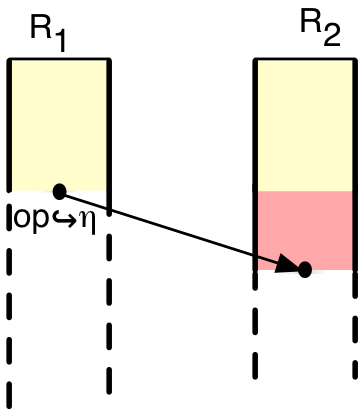
\includegraphics[scale=0.7]{Figures/ec-theirs}
 
}
\hspace*{0.1in}
\subcaptionbox {
  Subset model
  \label{fig:ec-ours}
}{
  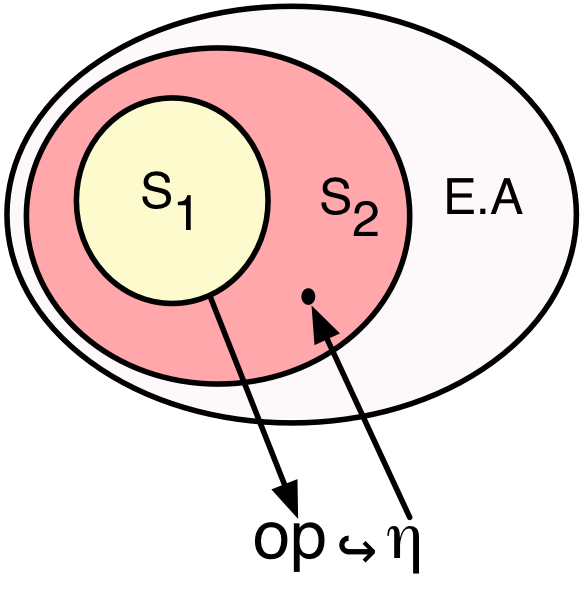
\includegraphics[scale=0.45]{Figures/ec-ours}
} \caption{In the replica model, operation $\op$ generates effect
$\eta$ at replica $R_1$, which is then merged to $R_2$. If the
\emph{store is {\sc cc}}, then $R_2$'s state at merge event is same or
larger than $R_1$'s state at generation event (the difference is
highlighted). In our subset model, $\op$ witnesses $S_1 \subseteq
\E.\A$ and generates $\eta$, which is immediately added to $\E.\A$. A
later operation may witness $S_2 \subseteq \E.\A$, and if the
\emph{operation is} {\sc cc} and $\eta \in S_2$, then it also
witnesses $S_1$ (i.e., $S_1 \subseteq S_2$). } 
% Moreover, Like $R_2 - R_1$, if all effects in $S_2 - S_1$ are
% concurrent with $\eta$, i.e., $\not\exists\eta'.~\eta' \in S_2 - S_1
% \conj % visZ(\eta,\eta')$, then any precondition $P$ that is valid
% when $\op$ executed is also valid when $\eta$ is witnessed because
% of the stability condition.
\label{fig:ec-theirs-vs-ours}
\end{figure}

Reasoning under weakly-consistent replication has received special
attention in recent work~\cite{gotsmanpopl16}. Our operational
semantics and proof system are general enough to admit replication as
a special case of our formulation. In this section, we explain how the
standard artifacts of weakly-consistent replication manifest in our
reasoning framework.

The primary challenge in this setting is to ensure that the
assumptions made and guarantees enforced by an operation at one
replica carry over to other replicas that merge their effects, thus
preserving the overall integrity of the system.  In prior
work~\cite{lbc16,gotsmanpopl16}, this challenge is partly addressed by
imposing restrictions on how various replica states differ, i.e., by
fixing a system model with a stronger baseline consistency ({\sc cc})
than {\sc ec}. This unfortunately restricts the reasoning approach
from being applied to data stores (e.g., \cite{bayou,pldi15}) that provide
guarantees weaker than causal consistency, such as causal visibility
or read-my-writes~\cite{zoo}. Causal consistency is not baseline
consistency in these stores because it is not \emph{highly
  available}~\cite{bailishat}.

Notably, our view of replication does not explicitly involve replicas.
Fig.~\ref{fig:ec-theirs-vs-ours} contrasts our model of
weakly-consistent replication with a conventional replica-based model.
Under our model, the notion of a replica is subsumed by the concept of
visibility; a replica is defined by the subset ($S$) of global state
($\E.\A$) that an operation witnesses. Constraints over replica states
therefore manifest as constraints over a specific visibility relation.
For example, instead of requiring the store to be causally consistent,
an operation can witness a causally consistent subset of the state;
such demands can be made via the trace invariant $\I$. For a
precondition ($P$) of the operation to be useful, it has to be an
assertion over every causally consistent subset of the global state.
Since any replica that eventually executes the operation has to expose
one such subset ($S$), the precondition is guaranteed to hold
regardless of the replica. There is however one problem with this
explanation - by considering subsets of just one global state, it
ignores the fact that the global state (hence, the replica states)
change during the execution of the operation. To account for such
changes, we might choose to distinguish between effect generation
event at one replica $r_1$ and effect merge event at replica $r_2$,
requiring that \emph{non-conflicting} operations execute between these
two events at $r_2$, and that they preserve certain
invariants~\cite{gotsmanpopl16}.  Instead, our framework folds all such
machinery into a stability condition predicated on $\I$
(\S\ref{sec:rely-guarantee}).  Since any change to the global state
during the execution of the operation is an interference, and $P$ is
required to be stable with respect to any such interference, it
follows that $P$ is valid on every replica, thus ensuring that
assumptions made at a generation event is also valid at the merge
event.

\subsection{Example}

We shall now consider the proof of the example in
Fig.~\ref{fig:motiv-eg-1} in greater detail. We assume an {\sc sc}
store, such as a relational database, whose store-specific trace
invaraint ($\I_s$) was shown previously. Both transactions are run at
{\sc si} isolation, hence $\I_c$ is $\lambda\E.~\underE{\C{SI(Wd1)}}
\conj \underE{\C{SI(Wd1)}}$. As usual, $\I$ is $\I_s \conj \I_c$. 

\begin{figure}
\centering
\begin{txnimpcode}
 $\begin{decoration}
 P_1:\{ {\neg\committed(\C{Wd2})} \Rightarrow \C{C = k} \conj\\
        \hspace*{0.3in}{\committed(\C{Wd2})} \Rightarrow \C{Wd2}
        \visar \C{Wd1} \wedge \C{Wd2} \wrstoar \C{C} \wedge \C{C = k-a2} \}
 \end{decoration}$
  txn$\langle$'Wd1'$\rangle${
   $\begin{decoration}
    \phi_1 : \{{\neg\committed(\C{Wd2})} \Rightarrow \C{C = k} \conj
      {\committed(\C{Wd2})} \Rightarrow \C{Wd2} \wrstoar \C{C} \conj\\
       \hspace*{0.3in}{\committed(\C{Wd2})} \wedge
        {\C{Wd2} \visar \C{Wd1}} 
       \Rightarrow \C{C = k-a2} \}
    \end{decoration}$ 
    v1 = C
   $\begin{decoration}
    \phi_2 : \{{\neg\committed(\C{Wd2})} \Rightarrow \C{C = k} \wedge \C{v1 = k} \conj\\
       \hspace*{0.3in}{\committed(\C{Wd2})} \Rightarrow \C{Wd2} \wrstoar \C{C} \conj \\
       \hspace*{0.3in}{\committed(\C{Wd2})} \wedge
        {\C{Wd2} \visar \C{Wd1}} 
       \Rightarrow \C{C = k-a2} \wedge \C{v1 = k-a2}\}
    \end{decoration}$ 
    if (v1 $\ge$ a1) {
      v2 = C;
     $\begin{decoration}
      \phi_3 : \{{\neg\committed(\C{Wd2})} \Rightarrow \C{C = k} \wedge \C{v2 = k} \conj\\
       \hspace*{0.3in}{\committed(\C{Wd2})} \Rightarrow \C{Wd2} \wrstoar \C{C} \conj \\
         \hspace*{0.3in}{\committed(\C{Wd2})} \wedge
          {\C{Wd2} \visar \C{Wd1}} \Rightarrow \C{C = k-a2} \wedge \\
          \hspace*{1.9in}\C{v2 = k-a2}\}
      \end{decoration}$ 
      v3 = v2 - a1;
     $\begin{decoration}
      \phi_4 : \{{\neg\committed(\C{Wd2})} \Rightarrow \C{C = k} \wedge \C{v3 = k-a1} \conj\\
         \hspace*{0.3in}{\committed(\C{Wd2})} \Rightarrow \C{Wd2} \wrstoar \C{C} \conj \\
         \hspace*{0.3in}{\committed(\C{Wd2})} \wedge
          {\C{Wd2} \visar \C{Wd1}} 
         \Rightarrow \C{C = k-a2} \wedge \\
         \hspace*{1.9in}\C{v3 = k-a2-a1}\}
      \end{decoration}$ 
      C := v3
     $\begin{decoration}
      \phi_5 : \{{\neg\committed(\C{Wd2})} \Rightarrow \C{C = k-a1}) 
                \conj\\
         \hspace*{0.3in}{\committed(\C{Wd2})} 
                \Rightarrow \C{C = k-a1-a2}\}
      \end{decoration}$ 
    }
  }
 $\begin{decoration}
  Q_1 : \{{\neg\committed(\C{Wd2})} \Rightarrow \C{C = k-a1}
            \conj \committed(\C{Wd1}) \conj\\
      \hspace*{0.12in}{\committed(\C{Wd2})} 
          \Rightarrow \C{C = k-a1-a2} \}
  \end{decoration}$ 
\end{txnimpcode}

\caption{\C{Wd1} transaction decorated with assertions}
\label{fig:wd1-decorated}
\end{figure}

The fully decorated implementation of transaction \C{Wd1} is shown in
Fig.~\ref{fig:wd1-decorated}. Decorated \C{Wd2} is similar and not
shown. Assignment statements are broken down and temporary local
variables (\C{v1}, \C{v2} and \C{v3}) are introduced so as to separate
shared variable reads and writes. All assertions implicitly refer to
the current execution ($\E$), just as hoare triples implicitly refer
to the current state. The context for propositions is also the
implicit, i.e., we write $\psi$ instead of $\underE{\psi}$. The
proposition \C{k $\ge$ a1+a2} remains an invariant, hence elided. The
precondition ($P_1$) of \C{Wd1} accounts for the possibility of
\C{Wd2} committing before \C{Wd1}, writing \C{k-a2} to \C{C}.
Precondition of \C{Wd2} is similar.  Since neither \C{Wd1} nor \C{Wd2}
are committed at the beginning, the execution-based assertion
corresponding to the precondition ($P$) of Fig.~\ref{fig:motiv-eg-1}
must include $\neg\committed(\C{Wd1}) \wedge \neg\committed(\C{Wd2})$,
from which $P_1$ follows. Once the execution is inside \C{Wd1}, commit
of \C{Wd2} ($\committed(\C{Wd2})$) may mean that either \C{Wd2}
happened before \C{Wd1} (hence can be visible to all of \C{Wd1}), or
that it committed concurrently with \C{Wd1} (hence cannot be visible
to all of \C{Wd2}).  Since SI proscribes the latter possibility, we
only consider the case when $\C{Wd2} \visar \C{Wd1}$. A proof for
$\C{Wd2} \visar \C{Wd1}$ is obtained subsequently, allowing us to get
rid of the special case.

First, we focus on the sequential aspect of the proof and show that
the assertions that decorate \C{Wd1} are indeed valid. The proof for
each triple follows from the rule for the corresponding term in
Fig.~\ref{fig:rg-rules}. For illustration, we consider the triple
corresponding to the assignment statement (line ??). The precondition
($\phi_4$) asserts that \C{Wd2} writes to \C{C}, and the value of the
temporary variable \C{v3} is \C{k-a2-a1}. The RG rule
(\rulelabel{RG-Asgn}) for assignment statement allows us to easiliy
conclude the following about the execution state after the assignment:

\begin{smathpar}
\begin{array}{l}
    {\neg\committed(\C{Wd1}) \conj \C{Wd1} \wrstoar \C{C} 
    \conj (\neg\committed(\C{Wd2})} \Rightarrow \C{C = k}) \conj\\
    ({\committed(\C{Wd2})} \Rightarrow \C{Wd2} \wrstoar
    \C{C}) \conj \\
    ({\committed(\C{Wd2})} \wedge {\C{Wd2} \visar \C{Wd1}} 
    \Rightarrow \C{C = k-a2} \wedge \C{C = k-a2-a1})
\end{array}
\end{smathpar}

\noindent The rule also lets us assume that the execution satisfies trace
invariant ($\I$), which asserts {\sc si} for both transactions.  Since
both transactions write to \C{C}, {\sc si} requires either $\C{Wd1}
\visar \C{Wd2}$, or $\C{Wd2} \visar \C{Wd1}$. Since \C{Wd1} is not yet
committed ($\neg\committed(\C{Wd1})$), {\sc si} prohibits the former
possibility, allowing us the deduce the $\C{Wd2} \visar \C{Wd1}$. This
lets us derive ${\committed(\C{Wd2})}  \Rightarrow \C{C = k-a2} \wedge
\C{C = k-a2-a1}$, allowing us to prove the postcondition ($\phi_5$).

The second part of the proof is to show that assertions are stable
despite the interference from the the concurrent thread executing
\C{Wd2}. The interference is given by the following rely relation
($R_1$):

\begin{smathpar}
\begin{array}{lcl}
  R_1 & = & \{ (\E,\E') \;|\; \neg\underE{\committed(\C{Wd2})} \conj 
        \underE{\I} \conj \E'\Vdash \I \conj\\
%       \conj (\E'-\E) \subseteq \C{Wd2} \conj \\
%   & & \hspace*{0.5in} \E' \Vdash \committed(\C{Wd2}) ~\Rightarrow~ \E'
%       \Vdash \C{Wd2} \wrstoar \C{C} \conj \\ 
%   & & \hspace*{0.5in} \underE{\committed(\C{Wd1})} \conj \E' \Vdash
%   \committed(\C{Wd2}) \Rightarrow \C{C=k-a1-a2} \\
    & & \hspace*{0.5in} \neg\underE{\committed(\C{Wd1})} \conj
        \C{COMMIT(Wd2)} \in (\E'-\E) \\
    & & \hspace*{0.8in}\Rightarrow \C{C=k-a2} \conj 
        \E' \Vdash \C{Wd2} \wrstoar \C{C} \conj \\
    & & \hspace*{0.5in} \underE{\committed(\C{Wd1})} \conj
        \C{COMMIT(Wd2)} \in (\E'-\E) \\
    & & \hspace*{0.6in}\Rightarrow \C{C=k-a1-a2} \conj
        \E' \Vdash \C{Wd2} \wrstoar \C{C} \}\\
\end{array}
\end{smathpar}

\noindent The rely relation says the following about the concurrent thread: (1).
It may interfere only if \C{Wd2} is not already committed, (2). Any
interference takes well-formed executions to well-formed executions,
(3). If the interference commits \C{Wd2}, then \C{Wd2} should have already
written to \C{C}, and (4). The value written is either $\C{k-a1-a2}$
or $\C{k-a1}$ depending on whether or not \C{Wd1} has already committed.
Stability for most assertions is straightforward. The only non-trivial
proof is for $\phi_5$, where {\sc si} condition should be used to
show that any interference from \C{Wd2} is invalid. The proof proceeds
on the same lines as the Hoare proof discussed above; it is also
discussed in \S\ref{sec:motivation}.

The final aspect of the proof is to show that any interference from
\C{Wd1} is contained in its guarantee relation $G_1$, which becomes
the rely relation ($R_2$) for \C{Wd2}. $R_2$ (hence $G_1$) is same as
$R_1$ shown above, but with \C{Wd2} and \C{Wd1} interchanged. $\ldots$


